\documentclass{beamer}

\usepackage{amsmath,amsthm, amssymb, latexsym}
\usepackage{subcaption}

% Theme stuff
\usetheme{Madrid}

\useinnertheme{circles}

% Define colors
\definecolor{color0}{RGB}{0,0,0} % black, for text
\definecolor{color1}{RGB}{128,0,0} % maroon, for titles, blocks
\definecolor{color2}{RGB}{118,118,118} % dark grey, for blocks
\definecolor{color3}{RGB}{255,253,250} % background color, white
\definecolor{color4}{RGB}{214,214,206} % light grey, title backgrounds
% Set colors for basic beamer elements
\setbeamercolor{headline}{bg=color4}
\setbeamercolor{footline}{bg=color4}
\setbeamercolor{block title}{bg=color4,fg=color1}
\setbeamercolor{frametitle}{bg=color4,fg=color1}
\setbeamercolor{title}{bg=color4,fg=color1}

\colorlet{beamer@blendedblue}{color1}

\newcommand{\T}{\frac{\theta}{2}}
\newcommand{\E}{\mathrm{E}}
\newcommand{\Var}{\mathrm{Var}}
\newcommand{\Cov}{\mathrm{Cov}}
\newcommand{\Pro}{\mathrm{P}}

%% \AtBeginSection[]
%% {
%%   \begin{frame}
%%     \frametitle{Table of Contents}
%%     \tableofcontents[currentsection]
%%   \end{frame}
%% }

\title[quant gen coal]{A general neutral model for quantitative trait
  distributions from a coalescent perspective}
\author{Evan Koch}
\date{August 5, 2017}

\begin{document}
\frame{\titlepage}
\frame{\tableofcontents}

\section{Introduction}

\subsection{Various models of neutral trait evolution}

\begin{frame}{Models of neutral trait evolution}
  \begin{itemize}
  \item Serve as null models for goodness of fit tests.
  \item Investigate the effects of demography and population structure in
    isolation.
  \end{itemize}
\end{frame}

\begin{frame}{Models of neutral trait evolution}
  \framesubtitle{Two extremes}
  \begin{columns}
    \begin{column}{0.48\columnwidth}
      \begin{block}{The long view ($t>>N_e$)}
        \includegraphics[width=\columnwidth]{long_div.pdf}
        \begin{itemize}
        \item {\footnotesize$Y_1 - Y_2 \sim N(0,2 t \sigma_m^2)$}
        \item Lande (1976)
        \end{itemize}
      \end{block}
    \end{column}
    \begin{column}{0.48\columnwidth}
      \begin{block}{The short view ($t<<N_e$)}
        \includegraphics[width=\columnwidth]{short_div.pdf}
        \begin{itemize}
        \item {\footnotesize$(Y_1,Y_2) \sim N(Y_A,
          \begin{pmatrix}
            f_{11} & f_{12}\\
            f_{12} & f_{22}
          \end{pmatrix}\sigma_A^2)$}
        \item Wright (1951)
        \end{itemize}
      \end{block}
    \end{column}
  \end{columns}  
\end{frame}

\begin{frame}{Looking for adaptive differentiation among populations}
  \framesubtitle{The $Q_{ST}$ paradigm}
  \begin{block}{Does $Q_{ST}$ exceed a neutral expectation?}
    \begin{equation*}
    Q_{ST} = \frac{V_{among}}{2V_{within}+V_{among}}
    \end{equation*}
  \end{block}
  Recent variations on this theme:
  \begin{itemize}
  \item Use GWAS hits to calculated genetic values and test for overdispersion
    (Berg and Coop, 2014)
  \item Full model of breeding experiments, population structure, and trait
    covariance (Ovaskainen et al., 2011)
  \end{itemize}
\end{frame}

\subsection{Trait models using the coalescent}

\begin{frame}{Few quantitative genetic models are coalescent-based}
  \begin{block}{Whitlock, 1999}
    Used coalescent argument to demonstrate that $\E[Q_{ST}]=\E[F_{ST}]$. 
  \end{block}
  \begin{block}{Griswold et al., 2007}
    Investigated the effects of shared ancestry and linkage disequilibrium on
    the genetic covariance matrix. 
  \end{block}
  \begin{block}{Schraiber and Landis, 2015}
    Use a coalescent model to show that the normality assumption can be violated
    when
    \begin{itemize}
    \item The number of loci affecting a trait is small.
    \item Mutational distributions are skewed or fat-tailed.
    \end{itemize}
  \end{block}
\end{frame}

\begin{frame}{The Schraiber and Landis model}
  \begin{columns}
    \begin{column}{0.55\columnwidth}
      \begin{center}
        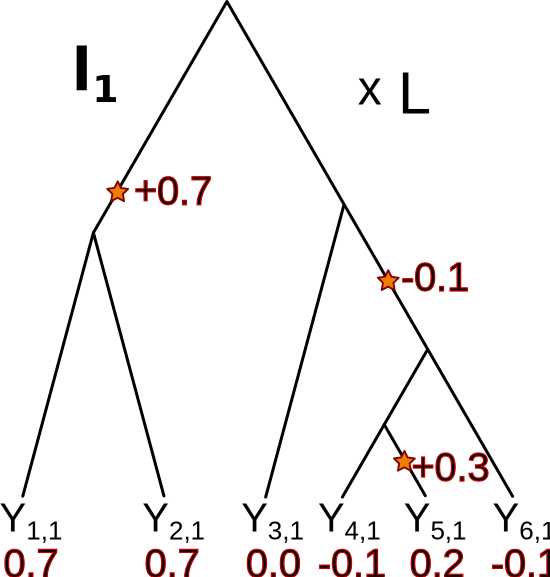
\includegraphics[width=0.9\columnwidth]{sl_model.pdf}
      \end{center}
    \end{column}
    \begin{column}{0.42\columnwidth}
      \begin{block}{Individual trait values}
        \begin{equation*}
          Y_i = \sum_{\ell=1}^L Y_{i,\ell}
        \end{equation*}
      \end{block}
      \begin{itemize}
      \item Sample size: $n$
      \item Mutation rate: $\T$
      \item Genealogies and mutational effects are both random variables.
      \item Stepping stone model of mutation within loci (Kimura, 1965).
      \end{itemize}
    \end{column}
  \end{columns}
\end{frame}

\subsection{Goals}

\begin{frame}{Goals}
  \begin{itemize}
  \item Extend Schraiber and Landis (2015) model to arbitrary genealogical
    distributions.
  \item How does the genealogical distribution influence deviations from
    normality?
  \item How do classical evolutionary quantitative genetics results fit into
    coalescent framework?
  \item What are the implications for selection tests?
  \end{itemize}
\end{frame}

\section{Results}

\subsection{The moment generating function of the trait value distribution}

\begin{frame}{The moment generating function for trait values}
  The moment generating function (mgf) for a sample of trait values is 
  \begin{definition}[Moment generating function]
    \begin{equation*}
      \varphi_{\mathbf{Y}}(\mathbf{k}) = \E\left[ e^{\mathbf{k} \cdot \mathbf{Y}} \right] =
      \int e^{\mathbf{k} \cdot \mathbf{Y}} \Pro(\mathbf{Y}=\mathbf{y}) \mbox{d}\mathbf{y}
    \end{equation*}
    \begin{itemize}
    \item $\mathbf{k}$ is a vector of dummy variables, one for each individual.
    \end{itemize}
  \end{definition}
  Schraiber and Landis found the moment generating function in the standard neutral model to be
  \begin{block}{}
    \begin{equation*}
      \varphi_{\mathbf{Y}}(\mathbf{k}) = \frac{2}{n(n-1) - \theta \left( \sum_{i=1}^n \varphi_{Y_i}(k_i) - n \right)}
      \sum_{i<j} \varphi_{\mathbf{Y}^{(i,j)}}(\mathbf{k}^{(i,j)})
    \end{equation*}
    \begin{itemize}
    \item $(i,j)$ indicates that samples $i$ and $j$ coalesce.
    \end{itemize}
  \end{block}
\end{frame}

\begin{frame}{The mgf for arbitrary demography}
  \begin{block}{Condition on the genealogy at a locus}
    \begin{align}
      \varphi_{\mathbf{Y}}(\mathbf{k}) &= \int e^{\mathbf{k} \cdot \mathbf{Y}}
      \int \Pro(\mathbf{Y}=\mathbf{y} | \mathbf{T}=\mathbf{t}) \Pro(\mathbf{T}=\mathbf{t})
      \mbox{d}\mathbf{t} \mbox{d}\mathbf{y}\\
      &= \int \int e^{\mathbf{k} \cdot \mathbf{Y}} \Pro(\mathbf{Y}=\mathbf{y} | \mathbf{T}=\mathbf{t}) \mbox{d}\mathbf{y}
      \Pro(\mathbf{T}=\mathbf{t})
      \mbox{d}\mathbf{t}
    \end{align}  
  \end{block}
  \begin{block}{Break up evolution along branches}
    \begin{itemize}
    \item $\Omega$: Set of all possible branches 
    \item $\omega$: A branch, a set containing all individuals subtended by the
      branch, e.g $\omega = (a,b,c)$.
    \end{itemize}
    \begin{equation*}
      \Pro(\mathbf{Y}=\mathbf{y}|\mathbf{T}=\mathbf{t}) = \prod_{\omega \in \Omega}
      \Pro(\mathbf{Y}_{\omega}=(y_{i,\omega})_{i \in \omega} | \mathbf{T}=\mathbf{t}).  
    \end{equation*}
  \end{block}
\end{frame}

\begin{frame}{The mgf for arbitrary demography}
  \begin{block}{Trait change is a compound Poisson process along branches}
    \begin{equation*}
        \exp\left( \frac{\theta}{2} t_{\omega} \left( \psi\left(\sum_{i \in \omega}k_{\omega}\right) -1 \right)\right).
    \end{equation*}
    \begin{itemize}
    \item $\psi$ is the mgf of the mutational distribution.
    \end{itemize}
  \end{block}
  \begin{block}{Putting this all together gives}
    \begin{align*}
      \varphi_{\mathbf{Y}}(\mathbf{k}) &= \prod_{\omega \in \Omega}
      \int \exp\left( \frac{\theta}{2} t_{\omega} \left( \psi\left(\sum_{a \in \omega}k_{a}\right) -1 \right)\right)
      \Pro(\mathbf{T}=\mathbf{t})\mbox{d}\mathbf{t} \\
      &=
      \varphi_{\mathbf{T}}(\mathbf{s})\Bigr|_{s_{\omega}=\frac{\theta}{2} \left( \psi\left(\sum_{a \in \omega}k_{a}\right) -1 \right)}.
    \end{align*}
    \begin{itemize}
    \item The trait mgf is obtained by making a substitution into the genealogy mgf.
    \end{itemize}
  \end{block}
\end{frame}

\begin{frame}{Genealogical mgfs}
  The Schraiber and Landis result can be obtained using an mgf previously
  derived by Lohse et al. 2011.
  \begin{block}{Genealogy mgf for a locus in a panmictic, constant-size population}
    \begin{equation*}
      \varphi_{T}(\mathbf{s}) = \frac{1}{n(n-1)/2 - \sum_{i=1}^n s_i}\sum_{i<j}\varphi_{\mathbf{T}^{(i,j)}}(\mathbf{s}^{(i,j)})
    \end{equation*}
  \end{block}
  With the substitution
  ${s_{\omega}=\frac{\theta}{2} \left( \psi\left(\sum_{a \in \omega}k_{a}\right) -1 \right)}$ we get
  \begin{block}{Schraiber and Landis result}
    \begin{equation*}
      \varphi_{\mathbf{Y}}(\mathbf{k}) = \frac{2}{n(n-1) - \theta \left( \sum_{i=1}^n \varphi_{Y_i}(k_i) - n \right)}
      \sum_{i<j} \varphi_{\mathbf{Y}^{(i,j)}}(\mathbf{k}^{(i,j)})
    \end{equation*}
  \end{block}
\end{frame}

\begin{frame}{Genealogical mgfs}
  Lohse et al. also derive the genealogy mgf for other cases:
  \begin{itemize}
  \item Populations connected by migration
  \item The IM model 
  \item Step changes in population size
  \item Recombination between loci
  \end{itemize}
  Writings recursions for different possible models is not particularly
  illuminating.
\end{frame}

\subsection{Low mutation rate approximations}

\begin{frame}{Population model details disappear in the low mutation rate limit}
  \begin{figure}
    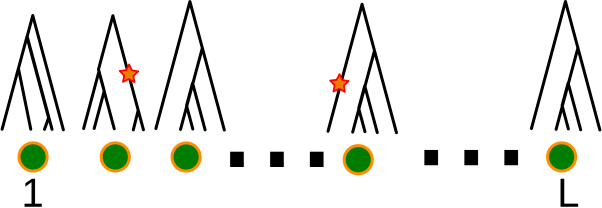
\includegraphics[width=\textwidth]{low_mut.pdf}        
  \end{figure}
\end{frame}

\begin{frame}{Population model details disappear in the low mutation rate limit}
  \begin{block}{Low mutation rate approximation}
    \begin{equation*}
      \varphi_{\mathbf{Y}}(\mathbf{k}) \approx \left[ 1 + \sum_{\omega \in \Omega}
        \E[T_\omega] \T \left( \psi\left( \sum_{a \in \omega} k_a\right) -1 \right) \right]^L.
    \end{equation*}
  \end{block}
  \begin{itemize}
  \item $t_\omega\left(\T\right)^2 \approx 0$
  \item Calculate moments in terms of expected internal branch lengths
  \item Also easy to derive from the expected site frequency spectrum
  \end{itemize}
\end{frame}

\begin{frame}{An example moment calculation: Kurtosis}
  \begin{definition}[Kurtosis]
    \begin{equation*}
      \mbox{Kurt}[X]=\frac{\E[(X-\E[X])^4]}{(\E[(X-\E[X])^4)^2}.
    \end{equation*}
  \end{definition}
  \begin{figure}
    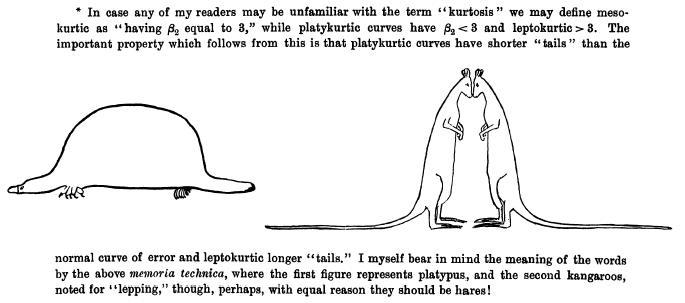
\includegraphics[width=\textwidth]{kurtosis-Student1927.png}        
  \end{figure}
\end{frame}

\begin{frame}{An example moment calculation: Kurtosis}
  For a panmictic population and a mutational distribution with zero mean and
  zero skew.
  \begin{block}{Expected population kurtosis}
    \begin{equation*}
      \E[\mbox{Kurt}] \approx 3 + \frac{\kappa( 4\E[T_2] - 6\E[T_3] + 
        3\E[T_4])}{L \T \E[T_2]}
    \end{equation*}
  \end{block}
  \begin{itemize}
  \item $\kappa$: kurtosis of the mutational distribution
  \item $\E[T_i]$L expected $T_{MRCA}$ for a sample of size $i$. 
  \end{itemize}
  \begin{block}{Constant-size population}
    \begin{equation*}
      3 + \frac{\kappa}{2L\T \E[T_2]}
    \end{equation*}
  \end{block}
\end{frame}

\subsection{The infinitesimal limit}

\begin{frame}{The infinitesimal (normal) model}
  \begin{itemize}
  \item Number of loci $\uparrow$
  \item Effect size of mutations $\downarrow$
  \end{itemize}
  \begin{block}{Infinitesimal limits}
    The following limits yield a normal distribution:
    \begin{columns}
      \begin{column}{.47\columnwidth}
        \begin{itemize}
        \item $L\T m_1 \to \mu$
        \item $L\T m_2\to \sigma^2$
        \end{itemize}
      \end{column}
      \begin{column}{.47\columnwidth}
        \begin{itemize}
        \item $L^i\left(\T\right)^j \to 0$ for $i<j$
        \item as $L \to \infty$
        \end{itemize}
      \end{column}
    \end{columns}
    \begin{equation*}
      \varphi_{\mathbf{Y}}(\mathbf{k}) = \exp \left( \sum_{\omega \in \Omega}\E[T_{\omega}] \left( \mu \left(
      \sum_{a \in \omega} k_a\right) + \frac{\sigma^2}{2}\left( \sum_{a \in \omega}
      k_a\right)^2\right)\right).
    \end{equation*}
    This is the mgf for a normal distribution with
    \begin{itemize}
    \item $\E[Y_a] = \E[T_{MRCA}] \mu$
    \item $\Var[Y_a] = \E[T_{MRCA}]\sigma^2$
    \item $\Cov[Y_a,Y_b] = (\E[T_{MRCA}] - \E[T_{a+b}]) \sigma^2$
    \end{itemize}
  \end{block}
\end{frame}

\begin{frame}{Relationship with previously used normal models}
  \framesubtitle{Deep divergence}
  \begin{figure}
    \includegraphics[width=0.4\columnwidth]{long_div.pdf}      
  \end{figure}
  \begin{equation*}
    \footnotesize
    (Y_1 , Y_2) \sim N(\E[T_{MRCA}] \mu \mathbf{1}, \sigma^2
    \begin{pmatrix}
      \E[T_{MRCA}] & (\E[T_{MRCA}] - \E[T_{1,2}])  \\
      (\E[T_{MRCA}] - \E[T_{1,2}]) & \E[T_{MRCA}]
    \end{pmatrix})
  \end{equation*}
  \begin{equation*}
    Y_1 - Y_2 \sim N(0, 2 \sigma^2 \E[T_{1,2}])
  \end{equation*}
  \begin{equation*}
    E[T_{1,2}] \approx t
  \end{equation*}
\end{frame}

\begin{frame}{Relationship with previously used normal models}
  \framesubtitle{Recent divergence}
  \begin{columns}
    \begin{column}{0.5\textwidth}
      \begin{figure}
        \includegraphics[width=\columnwidth]{short_div.pdf}   
      \end{figure}
    \end{column}
    \begin{column}{0.47\textwidth}
      \begin{equation*}
        (Y_1,Y_2) \sim N(Y_A,
          \begin{pmatrix}
            f_{11} & f_{12}\\
            f_{12} & f_{22}
          \end{pmatrix}\sigma_A^2)
      \end{equation*}
    \end{column}
  \end{columns}
\end{frame}

\begin{frame}{Conclusions}
  \begin{itemize}
  \item We can investigate the sampling distribution of trait values by first
    deriving or looking up the mgf for the genealogy.
  \item This is simplified considerably by only allowing one mutation per locus.
  \item Deviations from normality will depend on demography and population
    structure.
  \item We can connect neutral models for trait evolution at different levels of
    divergence.
  \end{itemize}
\end{frame}

\begin{frame}{Future directions}
  \begin{itemize}
  \item Incorporate recombination
  \item Relevance at intermediate levels of divergence where both mutation and
    drift should be modeled?
  \end{itemize}
\end{frame}

\begin{frame}{Acknowledgments}
  \begin{itemize}
  \item Funding: NSF GRFP
  \item Novembre lab members
  \item Midwest popgen conference organizers
  \end{itemize}
\end{frame}

\end{document}
